\chapter{Electromagnetic Worldlines: Numerical Forces and Curvatures
for the TE Polarization}
\label{ch:force}
The preceding work has focused on computing the Casimir energy between dielectric bodies.  However,
a number of experiments directly measure the force, or even the second spatial derivative of the energy.
Experiments that detect the shift in frequency of an oscillator, such as 
measuring the motion of a BEC in a harmonic trap~\cite{Harber2005,Obrecht2007}, or  
a nanoelectromechanical oscillators~\cite{Chan2001}, are sentitive the curvature of the Casimir energy.

As already noted in Sec.~\ref{sec:finite_difference}, the finite difference method has some drawbacks
when applied to worldline path integrals.  
Derivatives of discontinuous functions such as those required in worldline path integrals lead to large fluctuations.
In Sec.~\ref{sec:partial_averaging}, we developed specialized techniques for handling gradients of Casimir--Polder 
energies.  This chapter develops a parallel discussion for computing the force on macroscopic bodies.  

Prior investigations by Weber and Gies computed the Casimir force for
the Dirichlet worldline method~\cite{Weber2009, Weber2010}.
They computed the force between a planar surface and a cylindrical or spherical body, and the
torque between inclined plates.  Their methods typically rely on finding analytical expressions for 
when a particular Brownian path will intersect the surfaces, and analytically integrate over 
the path time and path starting position.  

In contrast, our approach to the worldline method has further emphasized Monte Carlo integration over
the path time and starting position.  
We have therefore developed worldline expressions to directly compute the force, potential curvature
and torque that apply between arbitrarily shaped bodies.  The resulting path integrals consider 
paths pinned to start on the surfaces of the bodies.  
The following results are explicitly derived for
the TE polarization, although presumably these results could be suitably generalized to the TM polarization.  

\section{Surface Pinned Paths}
\label{sec:path-pinning}

The renormalized TE Casimir energy was given in Eq.~(\ref{eq:TE_Casimir}). 
Although the energy was derived under the assumptions of describing electromagnetism in planar media,
it can be studied in its own right in arbitrary geometries of bodies, even if it cannot be 
strictly identified with the electromagnetic Casimir energy.    
We will consider the following worldline path integral
\begin{equation}
  E = \frac{\hbar c}{2(2\pi)^{D/2}}\int_0^\infty \frac{d\cT}{\cT^{1+D/2}}
  \, W,
  \label{eq:spatial_path_integralE}
\end{equation}
% Since we will be computing derivatives of the Casimir energy with respect to distance, and angle,
% we can confine our attention to just the spatial part of the integral, which is schematically given 
% by
where the spatial part of the worldline path integral is
\begin{align}
  W &:= \int d\vect{x}_0
  \,\biggdlangle \frac{1}{\langle\epsr\rangle^\alpha}-\frac{1}{[\epsr(\vect{x}_0)]^\alpha}\biggdrangle_{\vect{x}(t)},
  \label{eq:spatial_path_integral}
\end{align}
where $\alpha=1/2$ when applied to TE Casimir energies in planar geometries.    

In the following treatment 
we will consider a general geometry for computing Casimir forces between material bodies (Fig.~\ref{fig:spud_sketch}).
For simplicity, we will assume uniform dielectric bodies
separated by vacuum.  % , to focus on the most problematic features
% of sharp, dielectric interfaces.  However, the treatment here
% may be straightforwardly generalized to nonuniform dielectric media.
In this case, the relative dielectric permittivity $\epsr(\vect{r})$ is given  by 
\begin{equation}
  \epsr(\vect{r}) = 1+\sum_j\chi_j\Theta[\sigma_j(\vect{r}-\vect{R}_j)],
\end{equation}
where $\chi_j$ is the dielectric susceptibility of body $j$;
$\sigma_j(\vect{r})=0$ 
defines the surface of the $j$th body, with $\sigma_j>0$ and $\sigma_j<0$ 
on the interior and exterior of the body,
respectively; and $\vect{R}_j$ is the center of the $j$th body.  
\begin{figure}
  \centering
  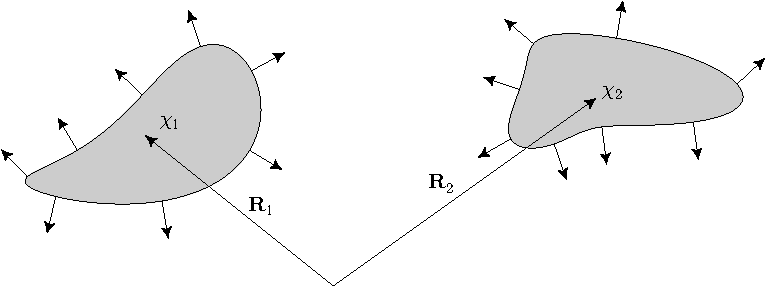
\includegraphics[width=0.6\columnwidth]{fig/spud_sketch}
  \caption[Sketch of geometry for interacting bodies]{
    Sketch of geometry for interacting dielectric bodies of susceptibility $\chi_j$, centered at
    $\vect{R}_j$ relative to the origin.  The surface of the $j$th body is
    defined by the condition $\sigma_j=0$.
    The normal vectors $\hat{n}_j$ to the surface of the $j$th  body
    are also shown.}
  \label{fig:spud_sketch}
\end{figure}

\subsection{Force}
The force on a body follows from the gradient of the Casimir energy,
where the derivatives are taken with respect to the body's 
position.
For example, the components of the force on body $2$, expressed
with Cartesian basis vectors $\hat{r}_i$, are
given by directional derivatives of the path integral in Eqs.~(\ref{eq:spatial_path_integral}) and 
(\ref{eq:spatial_path_integralE}) with respect to
the components of the body position $\mathbf{R}_2$:
\begin{align}
  &F_{2,i}:=-\frac{\hbar c}{2(2\pi)^{D/2}}\int_0^\infty \!\!\frac{d\cT}{\cT^{1+D/2}}\hat{r}_i\cdot\nablaR2 W
  \nonumber\\
   &\hspace{0.cm}=
   -\frac{\alpha\chi_2\hbar c}{2(2\pi)^{D/2}}
   \hat{r}_i\cdot\!\!
   \int_0^\infty \!\!\!\frac{d\cT}{\cT^{1+D/2}}   \!\int \!d\vect{x}_0\, 
  \Biggdlangle \frac{
  \big\langle 
  \delta(\sigma_2)\,\nabla\sigma_2\big\rangle}
  {\langle\epsr\rangle^{\alpha+1}}\Biggdrangle_{\!\vect{x}(t)}\!\!\!\!,
  \label{eq:forcepathint}
\end{align}
where $\sigma_2 = \sigma_2[\vect{x}(t)-\vect{R}_2]$ in this expression
, and $\nablaR{i}$ denotes the gradient with
respect $\vect{R}_i$.
The path-averaged $\delta$-function acts to pin the paths to the surface where $\sigma_2=0$.
% The path integration can be simplified by viewing the $\delta$-function,
% whose argument involves $\vect{x}(t)$, as a constraint on the
% source point $\vect{x}_0$ of the paths.
Writing out the relevant part of the path integral (\ref{eq:forcepathint}),
the $\delta$-function reduces the $D$-dimensional integration
over $\vect{x}_0$ to a $(D-1)$-dimensional integration over
the surface of body 2:
\begin{align}
  &\int d\vect{x}_0  \Biggdlangle \frac{
  \big\langle 
  \delta\big(\sigma_2[\vect{x}(t)-\vect{R}_2]\big)\,\nabla\sigma_2[\vect{x}(t)-\vect{R}_2]\big\rangle}
  {\langle\epsr\rangle^{\alpha+1}}\Biggdrangle_{\vect{x}(t)} \nonumber\\
  % &\hspace{0.5cm}= 
  % \int d\vect{x}_0  \Biggdlangle \frac{
  % \delta\big(\sigma_2[\vect{x}_0-\vect{R}_2]\big)\,\nabla\sigma_2[\x0-\vect{R}_2]}
  % {\langle\epsr\rangle^{\alpha+1}}\Biggdrangle_{\vect{x}(t)} \nonumber\\
  &\hspace{0.5cm}= 
  \oint\limits_{\sigma_2(\vect{x}_0-\vect{R}_2)=0}^{}
   \hspace{-3ex}
dS\hspace{1.5ex}\biggdlangle 
  \frac{\nabla\sigma_2(\x0-\vect{R}_2)}
  {\langle\epsr\rangle^{\alpha+1}|\nabla\sigma_2(\x0-\vect{R}_2)|}\biggdrangle_{\vect{x}(t)},
  \label{eq:delta-normal}
\end{align}
where the final integral (over path source points $\vect{x}_0$)
is a surface integral over the 
surface of body 2.  % The first equality here can be understood
% in terms of a discrete path (i.e., in a ``time-slicing'' regularization
% of the path integral), where the path average in the numerator
% amounts to a sum of terms, each involving a $\delta$-function
% involving a path coordinate $\vect{x}_j$.  In the average over all
% paths and sum over all source points $\vect{x}_0$,
% the $\delta$-function is equivalently a function of the
% source point, since $\vect{x}_j$ is the source point
% of another equivalent path.
This result follows from simplifying the path-averaged $\delta$-function using Eq.~(\ref{eq:delta_pin}),
and the following result~\cite{Hormander1983} 
\begin{equation}
  \int d\mathbf{x}\, \delta[h(\vect{x})]\,f(\vect{x})
  = \int_{h^{-1}(0)} \!\!\!\!\!dS_0\,\frac{1}{|\nabla h(\vect{x})|}f(\vect{x}),
  \label{hormander1}
\end{equation}
where $S$ is the surface satisfying $h(\vect{x})=0$, and 
\begin{equation}
|\nabla h(\vect{x})|=\Bigg[\sum_k \left(\frac{\partial h}{\partial x_k}\right)^2\Bigg]^{1/2}.
  \label{hormander2}
\end{equation}
% The 
% follows from an application of the H\"ormander formula
% (see Eq.~(22) in Ref.~\cite{Mackrory2016}).
The renormalized force vector can be found by summing over all force components, and subtracting 
the corresponding single-body force,
\begin{align}
  \vect{F}_{2}&=
  -\frac{\alpha\chi_2\hbar c}{2(2\pi)^{D/2}}
\int\limits_0^\infty \!\frac{d\cT}{\cT^{1+D/2}}    
\hspace{-3ex}
 \oint\limits_{\sigma_2(\vect{x}_0-\vect{R}_2)=0}^{}
  \hspace{-4ex} dS\hspace{1ex} 
  \hat{n}_2(\vect{x}_0) % \nonumber\\
  % &\hspace{0.5cm}\times 
  \Biggdlangle\frac{1}{\langle\epsilon_{\mathrm{r},12}\rangle^{\alpha+1}}-\frac{1}{\langle\epsilon_{\mathrm{r},2}\rangle^{\alpha+1}}
  \Biggdrangle_{\vect{x}(t)},
  \label{eq:pinning_force}
\end{align}
where the unit-normal vector for the surface of body 2 is defined by
\begin{equation}
  \hat{n}_2(\x0) := -\frac{\nabla \sigma_2(\x0-\vect{R}_2)}{|\nabla \sigma_2(\x0-\vect{R}_2)|}.
\end{equation}
Qualitatively, the Casimir force on a body arises from 
paths that start on a body's surface.  The direction of the 
force from a small patch of the surface is determined by the local
surface normal. 
Since each patch is at different distances from the other bodies, 
the paths from each patch contribute at different path times.  Once the integral 
over the surface is carried out, this results in a net force on the body.  

\subsection{Potential Curvature}

This method can be easily extended to the second derivative of the worldline energy, which 
computes the potential curvature,  
\begin{equation}
  C_{ij} := (\hat{r}_i\cdot \nablaR2)(\hat{r}_j\cdot \nablaR2)E.
\end{equation}
For a dielectric describing two bodies, the derivatives with respect to $\vect{R}_2$ in direction $\hat{r}_i$, can be rewritten 
in terms of derivatives with respect to the first body's center $\vect{R}_1$, and the loop coordinates $\vect{x}_k$
\begin{align}
  \nablaR2\langle \epsr\rangle  
  =& \bigg(\sum_{k=1}^N\nablaxk-\nablaR1\bigg)% \nonumber\\
  % & \times
[\langle \epsilon_1(\vect{x}-\vect{R}_1)\rangle+\langle\epsilon_2(\vect{x}-\vect{R}_2)\rangle],
% \frac{\partial}{\partial R_{2,i}}\langle \epsr\rangle  
%   =& \bigg(\sum_{k=1}^N\frac{\partial}{\partial {x}_{k,i}}-\frac{\partial}{\partial R_{1,i}}\bigg)\nonumber\\
%   & \times[\langle \epsilon_1(\vect{x}-\vect{R}_1)\rangle+\langle\epsilon_2(\vect{x}-\vect{R}_2)\rangle],
  \label{eq:shift_derivative}
\end{align}
where $\nablaxk$ is the gradient of the path position $\vect{x}_k$.    
The first derivative can be carried out as before,
\begin{align}
  C_{ij} = &
\frac{\alpha\chi_1\hbar c}{2(2\pi)^{D/2}}\intzinf \frac{d\cT}{\cT^{1+D/2}}
\int d\vect{x}_0 
\biggdlangle 
\hat{r}_{i}\!\cdot\!\bigg(\!\sum_k\nablaxk - \nablaR{1}\!\bigg)
  \!
  \frac{\big[\hat{r}_{j}\cdot\langle \nabla\sigma_2\delta(\sigma_2)\rangle\big]}
  {\langle\epsr\rangle^{\alpha+1}}\biggdrangle_{\vect{x}(t)}.
\end{align}

% \begin{align}
%   C_{ij} = &
% \frac{-\alpha(\alpha+1)\chi_2\hbar c}{2(2\pi)^{D/2}}\intzinf \frac{d\cT}{\cT^{1+D/2}}
% \int d\vect{x}_0 % \nonumber\\
% % &\hspace{0.05cm}\times
% \biggdlangle 
% \big(\hat{r}_{i}\cdot\langle \delta(\sigma_1)\nablaR{1}\sigma_1\rangle\big)\,\big(\langle \delta(\sigma_2)\nablaR{2}\sigma_2\rangle\cdot\hat{r}_{j}\big)
%   \frac{1}
%   {\langle\epsr\rangle^{\alpha+2}}\biggdrangle_{\vect{x}(t)}.
% \end{align}
It is possible to integrate by parts on the gradient $\nablaxk$, 
which then acts on the Gaussian probability density,
 and yields a term proportional to ${\sum_{k}(\vect{x}_k-\vect{x}_{k+1})}$.
This sum of path increments vanishes for closed paths, and thus this term can be dropped.  
The remaining gradient in $\nablaR{1}$ can be straightforwardly evaluated, which yields 
a second independent path-averaged $\delta$-function.  
\begin{align}
  C_{ij} = &
\frac{\alpha(\alpha+1)\chi_1\chi_2\hbar c}{2(2\pi)^{D/2}}\intzinf \frac{d\cT}{\cT^{1+D/2}}
\int d\vect{x}_0 % \nonumber\\
% &\hspace{0.05cm}\times
\biggdlangle 
\frac{\big[\hat{r}_{i}\cdot\langle \delta(\sigma_1)\nabla\sigma_1\rangle\big]\,
\big[\langle \delta(\sigma_2)\nabla\sigma_2\rangle\cdot\hat{r}_{j}\big]}
  {\langle\epsr\rangle^{\alpha+2}}\biggdrangle_{\vect{x}(t)}.
\end{align}
% and using Eq.~(\ref{eq:delta-normal}), there are now two path-averaged delta-functions which 
% pin the paths to lie on both the first and second surfaces
One $\delta$-function can be manipulated as in Eq.~(\ref{eq:delta-normal}) to constrain the paths to start on
the first body, while the second path-averaged $\delta$-function pins another point of the path to lie on the second body
and takes a further average over which point is pinned.
The resulting expression for the potential curvature is 
\begin{align}
  C_{ij}&=
  \frac{\alpha(\alpha+1)\chi_1\chi_2}{2(2\pi)^{D/2}}\intzinf \frac{d\cT}{\cT^{1+D/2}}
  \hspace{-2ex}
  \oint\limits_{\sigma_1(\vect{x}_0-\vect{R}_1)=0}^{}
   \hspace{-4ex} dS\hspace{1ex} %   \nonumber\\
  % &\hspace{0.5cm} \times 
  \frac{1}{N} \sum_{k=1}^{N-1} \,
  \oint\limits_{\sigma_2(\vect{x}_k-\vect{R}_2)=0}^{}
   \hspace{-4ex} dS_k\hspace{1ex} 
  \nonumber\\ 
&\hspace{1cm}\times
 \biggdlangle  \mathcal{G}(\vect{x}_0-\vect{x}_k,k(N-k)\cT/N^2)
  \frac{[\hat{r}_{i}\cdot\hat{n}_1(\vect{x}_0)][\hat{r}_{j}\cdot\hat{n}_2(\vect{x}_k)]}
  {\langle \epsilon_{\mathrm{r},12}\rangle^{\alpha+2}}     \biggdrangle_{\sigma_2(\vect{x}_k-\vect{R}_2)=0}.
  \label{eq:potential_curvature}
\end{align}
where 
$\dlangle \cdots\drangle_{\sigma_2(\vect{x}_k-\vect{R}_2)=0}$ is the ensemble
average over discrete paths $\vect{x}(t)$ subject to the constraint that $\sigma_2(\vect{x}_k-\vect{R}_2)=0$.
The $D$-dimensional Gaussian probability density
\begin{equation}
  \mathcal{G}(\vect{x},\sigma^2)=\frac{e^{-(\vect{x})^2/(2 \sigma^2)}}{[2\pi \sigma^2]^{D/2}},
  \label{eq:Gauss_normalization}
\end{equation}
has been used to write the combined normalization factor from fixing $\vect{x}_k$ after $k$ steps, and returning to $\vect{x}_0$
in $N-k$ steps. 
There is no need for any further renormalization, since this expression is only non-zero in the presence 
of both bodies, and $\mathcal{G}$ exponentially cuts off the integral at small $\cT$.    

% The pinning can be expressed for continuous paths as
% \begin{align}
%   C_{ij}&=
%   \frac{\alpha(\alpha+1)\chi_1\chi_2}{2(2\pi)^{D/2}}\intzinf \frac{d\cT}{\cT^{1+D/2}}\int_0^\cT \frac{d\tau}{\cT}% \nonumber\\
%   % &\times
%   \oint\limits_{\sigma_1[\vect{x}(0)]}^{}   \hspace{-2ex} dS
%   \oint\limits_{\sigma_2[\vect{x}(\tau)]}^{}  \hspace{-2ex} dS'\hspace{1ex}   
% \mathcal{G}'[\vect{x}(0),\vect{x}(\tau),\tau,\cT] \nonumber\\
%    &\hspace{1cm}\times
%   \biggdlangle\frac{\{\hat{r}_{i}\cdot\hat{n}_1\big[\vect{x}(0)\big]\}
%     \{\hat{r}_{j}\cdot\hat{n}_2\big[\vect{x}(\tau)\big]\}}
%   {\langle \epsilon_{\mathrm{r},12}\rangle^{\alpha+2}}     \biggdrangle_{\vect{x'}(t); \vect{x'}(\tau)},
% \end{align}
% where the ensemble average is over paths $\vect{x'}(\tau)$ that are 
% pinned to lie on surface $\sigma_1, \sigma_2$ at path positions
% $\vect{x}(0), \vect{x}(\tau)$ respectively.  The Gaussian normalization is 
% \begin{equation}
%   \mathcal{G}'[\vect{x}(0),\vect{x}(\tau),\tau,\cT]=\frac{\sqrt{\cT}}{\sqrt{2\pi  \tau(\cT-\tau)}}
%   e^{- \cT[\vect{x}(0)-\vect{x}(\tau)]^2/[2 \tau(\cT-\tau)]}
% \end{equation}

\subsection{Torque}
The torque on a body can be found from the first order variation in the energy as that body is
infinitesimally rotated about some axis.  
For concreteness, consider perturbing the dielectric by rotating the second body about its center
by angle $\phi$ about axis $\hat{m}$,
% \begin{equation}
%   K_m = -\partial_\phi W,
% \end{equation}
%where the perturbed dielectric is 
\begin{equation}
  \epsr(\vect{x}) = 1+\chi_1\Theta[\sigma_1(\vect{x}-\vect{R}_1)]
  +\chi_2\Theta\big\{\sigma_2[\mathcal{R}(\phi)(\vect{x}-\vect{R}_2)]\big\}.
\end{equation}
% where the second body has undergone an infinitesimal rotation 
% by an angle $\phi$ about an axis $\hat{m}$ about its center.  
The infinitesimal rotation matrix is given by 
\begin{equation}
  \mathcal{R}_{ij}(\phi) = \delta_{ij} - m_k\epsilon_{ijk}\phi +\order(\phi^2),
\end{equation}
where $\delta_{ij}$ is the Kronecker delta, and $\epsilon_{ijk}$ is the antisymmetric Levi-Civita tensor. 
Throughout this section there are implicit sums over repeated indices.    
The torque for a rotation about axis $\hat{m}$ can be written as $K_m:=\hat{m}\cdot\vect{K}=-\partial_\phi E$.
The $\phi$-derivative only acts on the path-averaged dielectric part of the energy integral,
\begin{align}
  \partial_\phi\langle\epsilon\rangle&=
  \chi_2\langle \partial_\phi\mathcal{R}_{ij}(\phi)(\vect{x}-\vect{R}_2)_j[\hat{r}_i\cdot\nabla\Theta(\sigma_2)]\rangle\nonumber\\
%  =-\chi_2\langle m_k\epsilon_{kij}(\vect{x}-\vect{R}_2)_j[\hat{r}_i\cdot\nabla\Theta(\sigma_2)]\rangle\nonumber\\
  &=\chi_2\hat{m}\cdot\langle (\vect{x}-\vect{R}_2)\wedge\nabla\Theta(\sigma_2)\rangle,
\end{align}
where we used the form of the infinitesimal rotation to write the result as a cross product\footnote{
We use the wedge operator $\wedge$ to denote the vector cross product to avoid confusion with
the traditional multiplication sign $\times$, which is used to denote multi-line multiplication throughout this
thesis.}
via $(\vect{a}\wedge\vect{b})_i=\epsilon_{ijk}a_jb_k$.  
This derivative can be directly substituted into the full torque path integral, 
and similar manipulations to Eq.~(\ref{eq:delta-normal}) can be carried out
to pin the paths to start on the surface of the second body.
In addition, given the form of $\partial_\phi\langle\epsr\rangle$ the full torque $\vect{K}$
can be found by identifying $\partial_\phi E=\hat{m}\cdot\vect{K}$.  
The full renormalized torque worldline path integral is 
\begin{align}
  \vect{K} &= \frac{\alpha\hbar c\chi_2}{2(2\pi)^{D/2}}\intzinf \frac{d\cT}{\cT^{1+D/2}} 
  \hspace{-3ex}
  \oint\limits_{\sigma_2(\vect{x}_0-\vect{R}_2)=0} 
   \hspace{-4ex} dS\hspace{1ex}\!\big[(\vect{x}_0-\vect{R}_{2})\! \wedge \!\hat{n}_2(\vect{x}_0)\big]   % \nonumber\\
  % &\hspace{0.5cm}\times
  \biggdlangle 
\frac{1}{\langle \epsilon_{\mathrm{r},12}\rangle^{\alpha+1}}
  -\frac{1}{\langle \epsilon_{\mathrm{r},2}\rangle^{\alpha+1}}\biggdrangle_{\vect{x}(t)}.
\end{align}
This has a strikingly similar form to the force path integral~(\ref{eq:pinning_force}).  
Here the integrand is weighted by the cross product of the vector from the body's center the surface,
and the surface normal. 
If the spatial integrand in Eq.~(\ref{eq:pinning_force}) is loosely interpreted as a force density,
then the torque integrand for each patch of the surface can interpreted as the local torque density.
This is in direct analogy with the expression for the torque $\vect{K}=\vect{r}\wedge \vect{F}$ from classical mechanics.

\subsection{Casimir--Polder Force}

We briefly note that an alternative expression for the Casimir--Polder force on an atom near a surface
can be found in analogy to the potential curvature in Eq.~(\ref{eq:potential_curvature}).
The force on the atom due to the TE Casimir effect is $F\supTE\subCPi = -\hat{r}_i\cdot\nabla_{\rA}V\subCP\supTE$.
  In Sec.~\ref{sec:partial_averaging} the derivatives of the path integral were taken directly,
  and the dominant contribution to the derivative came from from the Gaussian probability distribution.  
  Alternatively, one can change the coordinates to $\vect{x}(t)=\rA+\vect{y}(t)$, where 
  $\vect{y}(t)$ is a Brownian bridge starting and returning to the origin, $\vect{y}(0)=\vect{y}(\cT)=0$,
  and then take the desired derivatives.
  The resulting force expression is
\begin{align}
  F_i\supTE \!=&\! -\frac{\hbar c\alpha_0}{4(2\pi)^{D/2}}\intzinf \frac{d\cT}{\cT^{1+D/2}}\biggdlangle 
  \hat{r}_i\!\cdot\!\nabla_{\rA}\langle\epsr\rangle^{-3/2}
  \biggdrangle_{\vect{y}(t)},
\end{align}
where this path integral considers the change in energy as the whole path is translated,
while the results in Sec.~\ref{sec:partial_averaging}
correspond to shifting only the origin of the path, while keeping the rest of the path fixed.
The derivatives can be carried out, which for piece-wise constant media create $\delta$-functions.
In analogy with the potential curvature, since the starting point is fixed, it is necessary to 
average over pinning other path points to lie on the dielectric surface for each of the bodies.  
The Casimir--Polder force, after summing over all force components, is 
\begin{align}
  \vect{F}\supTE\subCP&=-\frac{3\hbar c\alpha_0}{8(2\pi)^{D/2}}
  \sum_{i=1}^{N_b}\sum_{k=1}^{N-1}\frac{\chi_i}{N}\intzinf \frac{d\cT}{\cT^{1+D/2}}
  \hspace{-3ex}
  \oint\limits_{\sigma_i(\vect{x}_k-\vect{R}_i)=0} 
   \hspace{-4ex} dS_k\hspace{1ex}
   \nonumber\\
   &\hspace{0.5cm} \times 
   \biggdlangle \mathcal{G}\big[\rA-\vect{x}_k,k(N-k)\cT/N^2\big]
   \frac{\hat{n}_i(\vect{x}_k)}
  {\langle \epsr\rangle^{5/2}} \biggdrangle_{\sigma_i(\vect{x}_k-\vect{R}_i)=0}.
\end{align}
 where we have reverted to using $\vect{x}(t)$, and $\mathcal{G}$ is given by 
 Eq.~(\ref{eq:Gauss_normalization}).%, and $i$ indexes each of the $N_b$ dielectric bodies.
In this method the paths are constrained to touch the bodies, which must be taken into account numerically
by averaging over paths where each index that is constrained.
In contrast, the Hermite-Gaussian method discussed in Sec.~\ref{sec:partial_averaging} 
uses the same paths regardless of the dielectric background.
While the path-pinning method requires more complicated path generation,
it does not suffer from diverging fluctuations as the path resolution is increased.
The Gaussian factor $\mathcal{G}$ exponentially suppresses contributions from pinning small indices $k$,
which would be the problematic terms as $\Delta \cT\rightarrow 0$, 
and thus this method does not require careful handling as $N$ increases.  

\section{Occupation Number}
\label{sec:occupation}

The preceding methods offer an intuitive picture of the Casimir force,
however they are poorly behaved in the strong-coupling limit.  
For a typical path of $N$ steps pinned to the surface, approximately half 
of the path will lie inside the body.  For $\chi\gg N$, the denominator $\langle\epsr\rangle^{-1/2}$ dominates
the integrand, so the estimated derivatives tend to zero as $\chi^{-1/2}$ for almost all paths.  
Only rare paths which start on the surface, but do not enter the bulk of the body will contribute significantly.  
As a result, the numerically estimated force goes to zero in the strong-coupling limit.
In this section we develop alternative expressions which are better behaved in the strong-coupling
limit and makes direct contact with prior work on Dirichlet worldlines.  

The spatial path integral can be written in exponential form via the Gamma function,
\begin{align}
  W &= \frac{1}{\Gamma[\alpha]}\int d\vect{x}_0 \int ds\, s^{\alpha-1}e^{-s}% \nonumber\\
  % &\hspace{0.5cm}\times
  \bigdlangle e^{-\langle \sum_i\chi_i\Theta_i(\vect{x})\rangle}
  - e^{-\sum_i\chi_i\Theta_i(\vect{x}_0)}\bigdrangle_{\vect{x}(t)}\label{eq:W_exp2}
\end{align}
where we have introduced a shorthand notation $\Theta_i(\vect{x}) = \Theta(\sigma_i[\vect{x}-\vect{R}_i])$.
The exponential spatial path integral for two bodies, after the single-body expressions have been factored out can 
be factorized as 
\begin{align}
  W &= \frac{1}{\Gamma[\alpha]}\int d\vect{x}_0 \int ds\, s^{\alpha-1}e^{-s}% \nonumber\\
  % &\hspace{0.5cm}\times
  \Bigdlangle 
  (e^{-\langle \chi_1\Theta_1(\vect{x})\rangle}-1)(e^{-\langle \chi_2\Theta_2(\vect{x})\rangle}-1) \nonumber\\
   &\hspace{1.25cm}
  -(e^{- \chi_1\Theta_1(\vect{x}_0)}-1)(e^{-\chi_2\Theta_2(\vect{x}_0)}-1)\Bigdrangle_{\vect{x}(t)}
\end{align}
The exponential of the path-averaged potential can be written as a product of potentials 
for each increment, and the potential can be simplified for step function dielectrics,
\begin{align}
  e^{-s \langle\chi_i\Theta_i(\vect{x})\rangle}= \prod_{k=0}^{N-1}
  \left[1+\Theta_i[\vect{x}_k](e^{-s\chi_i/N}-1)\right].\label{eq:exp_step_limit1}
\end{align}
% This way of regularizing the surface leads to 
% a different representation for the gradients of the Casimir energy.
% In this section, we are assuming the step-function is arbitrarily sharp, and taking that limit before any gradients are taken.  
% The gradient for a single position can be computed from Eq.~(\ref{eq:exp_step_limit1}) as
% \begin{align}
%   [\nablaxk e^{-s \chi_i\Theta_{b,k}/N}]_{\text{occupation}} 
% =& \delta_{b,k}(e^{-s\chi_i/N}-1)\vect{n}_i(\vect{x}_k)
%     \label{eq:occupation-grad}
% \end{align}
% where $\delta_{b,k} := \delta[\sigma_i(\vect{x}_k-\vect{R}_i)]$ and the un-normalized surface normal is
% $\vect{n}_i(\vect{x}_k):=\nabla\sigma_{b}(\vect{x}_k-\vect{R}_i)$.
(The results in Sec.~\ref{sec:path-pinning} can be recovered when $\chi/N\ll 1$. )
% In essence, that calculation assumed the step was the limit of a smooth sigmoidal function 
% and that the path had arbitrarily fine resolution on the scale over which the step-function jump occured,
% so that the gradient follows from applying the chain-rule, 
% \begin{align}
%   [\nablaxk e^{-s \chi_i\Theta_{b,k}/N}]_{\text{pinning}} 
%  =& \frac{s\chi_i}{N} \delta_{b,k}e^{-s \chi_i\Theta_{b,k}/N}\vect{n}_i(\vect{x}_k)
%   \label{eq:pinning-grad}
% \end{align}
% However, throughout this section we will treat using Eq.~(\ref{eq:occupation-grad}) to evaluate gradients,
% and later show how the earlier results are recovered.

The force on the second body can be computed by differentiating
the energy with respect to the body position $\vect{R}_2$.  The spatial part of the force integral
can be defined as
\begin{align}
  W_{F,2} :=& -\nablaR{2}W\\
  =& -\frac{1}{\Gamma[\alpha]}\int d\vect{x}_0\int ds\,s^{\alpha-1}e^{-s}\biggdlangle 
\bigg(1-\prod_{n=0}^{N-1}\left[1+\Theta_{1}(\vect{x}_k)(e^{-s\chi_1/N}-1)\right]\bigg)
  \nonumber\\
  &\!\times\sum_{j=0}^{N-1}\big(e^{-s\chi_2/N}-1\big)\vect{n}_2(\vect{x}_j)\delta[\sigma_2(\vect{x}_k-\vect{R}_2)]
  \prod_{k\ne j}\left[1+\Theta_{2}(\vect{x}_k)(e^{-s\chi_2/N}-1)\right]%\nonumber\\
  \!\biggdrangle_{\vect{x}(t)}.
\end{align}
where the constant term has zero derivative.
The integral over $s$ can be carried out more easily if the integrand is re-arranged into terms with 
a definite number of points $n$ inside each body $i$.  
We define the indicator functions
\begin{align}
  \I[i]0&:= \prod_{j=0}^{N-1}\bar{\Theta}_{i}(\vect{x}_j)\\
  \I[i]n&:= \sum_{j_1=1}^{N-1}\sum_{j_2>j_1}\cdots\sum_{j_{n}>j_{n-1}}\Theta_{i}(\vect{x}_{j_1})\Theta_{i}(\vect{x}_{j_2})
  \cdots\Theta_{i}(\vect{x}_{j_n}),
 \quad n\ge 1,
\end{align}
where $\I[b]n=1$ when there are exactly $n$ points inside body $i$, and zero otherwise;  
there are $n$ sums over indices $j_{n}$, each of which terminates at $j_n=N$.  
There are further restrictions on which of these terms contribute in the integrand.
Due to the presence of the $\delta$-functions, only $N-1$ points are free to 
enter the bodies.  This further implies that the number of points inside both bodies must be less than $N-1$. 
Finally, due to the renormalization, only paths with at least one point inside the first body contribute.  
Using the indicator functions, the re-arranged spatial path integral for the force is 
\begin{align}
  W_{F,2} =& (-1)\int d\vect{x}_0\int ds\,s^{\alpha-1}e^{-s}\biggdlangle \sum_{j=0}^{N-1}\hat{n}_2(\vect{x}_j)\delta_{2,j}\nonumber\\
  &\times\sum_{n=0}^{N-1}
  \big(e^{-s(n+1)\chi_2/N}-e^{-sn\chi_2/N}\big)\I[2]n\nonumber\\
  &\times \sum_{m=1}^{N-n-1}\big(1- e^{-s m \chi_1/N} \big)\I[1]m
  \biggdrangle_{\vect{x}(t)},
\end{align}
The $s$ integral can be carried out term by term, and the $\delta$-function can be used to pin paths onto the surface,
where the cyclic-permutation invariance of the path can be used to remove the path-average over pinning, 
as in Eq.~(\ref{eq:delta-normal}).
The full force path integral is given by 
\begin{align}
  \vect{F}_1 &= -\frac{\hbar c N}{2(2\pi)^{D/2}}\intzinf \frac{d\cT}{\cT^{1+D/2}}
  \oint\limits_{\sigma_2(\vect{x}_0-\vect{R}_2)=0}  \hspace{-4ex} dS_0
  \hspace{1.5ex}\hat{n}_2(\vect{x}_0)%  \nonumber\\
  % &\hspace{0.5cm}\times 
  \sum_{m=0}^{N-1}\,\sum_{n=1}^{N-m-1}\Bigdlangle
  \I[1]m\I[2]n f_{m,n}\Bigdrangle_{\vect{x}(t)},
  \label{eq:occupation_force}
\end{align}
% \begin{align}
%   \vect{F}_2 =& (-1)\frac{\hbar c N}{2(2\pi)^{D/2}}\intzinf \frac{d\cT}{\cT^{1+D/2}}
%   \hspace{-2ex}\oint\limits_{\sigma_2(\vect{x}_0-\vect{R}_2)=0}  \hspace{-4ex} dS
% % \nonumber\\
% %   &\hspace{0.5cm}\times 
%   \,\,\sum_{n=0}^{N-1}\sum_{m=1}^{N-n-1}\bigdlangle\hat{n}_2(\vect{x}_0)
%   \I[1]m\I[2]n f_{m,n}\bigdrangle_{\vect{x}(t)}
%   \label{eq:occupation_force}
% \end{align}
where the material dependence is carried by 
\begin{align}
  f_{m,n}&:=c_{m,n}-c_{m,n+1}-c_{0,n}+c_{0,n+1},\\
  c_{m,n} &:= \bigg( 1 + \frac{m\chi_1+n\chi_2}{N}\bigg)^{-\alpha},
\end{align}
which come from computing the change in the renormalized energy integrand as another point enters
the second body.  When $\chi_2/N\ll 1$, $f_{m,n}$ can be expanded to leading order in $\chi_2/N$, 
to recover our earlier results for the force.

In this result, the indicator functions carry the position dependence based on whether a given number of points are 
within each body, while $f_{n,m}$ carries the dependence on material properties based on the number of points inside each body.  
This expression is well-behaved in the $\chi\rightarrow\infty$ limit, where only 
the $n=0, m>0$ terms contribute.  In the strong-coupling limit, the main contribution to the 
force comes from paths that just graze the second surface, while also entering the first body.  

For completeness we note the analogous expressions for the torque and potential curvature.  
The manipulations and reasoning used in Sec.~\ref{sec:path-pinning} for the torque and potential curvature
apply here---the only difference is the form chosen for the gradient, 
and using the indicator functions in the integrand.  
The torque path integral is 
\begin{align}
  \vect{K}_1 =& -\frac{\hbar c N}{2(2\pi)^{D/2}}\intzinf\frac{d\cT}{\cT^{1+D/2}}
 \oint\limits_{\sigma_2(\vect{x}_0-\vect{R}_2)=0}  \hspace{-4ex} dS_0
  % \nonumber\\
  % &\times
  \sum_{m=0}^{N-1}\sum_{n=1}^{N-m-1}   \nonumber\\
  &\hspace{2.5cm} \times\Bigdlangle(\vect{x}_0-\vect{R}_2)\wedge\hat{n}_2(\vect{x}_0)\I[1]m \,\I[2]n\,  f_{m,n}\Bigdrangle_{\vect{x}(t)}.
\end{align}
% \begin{align}
%   \vect{K}_2 =& -\frac{\hbar c N}{2(2\pi)^{D/2}}\intzinf\frac{d\cT}{\cT^{1+D/2}}
%   \hspace{-2ex}\oint\limits_{\sigma_2(\vect{x}_0-\vect{R}_2)=0}  \hspace{-4ex} dS
%   % \nonumber\\
%   % &\times
%   \sum_{n=0}^{N-1}\sum_{m=1}^{N-n-1}
%   \Bigdlangle(\vect{x}_0-\vect{R}_2)\wedge\hat{n}_2(\vect{x}_0) % \nonumber\\
%   % &\hspace{2.5cm} \times
%   \I[1]m \I[2]n  f_{n,m}\Bigdrangle_{\vect{x}(t)}.
% \end{align}
The potential curvature is given by
\begin{align}
  C_{ij} =& \frac{\hbar c N}{2(2\pi)^{D/2}}\sum_{k=1}^{N-1}\intzinf\frac{d\cT}{\cT^{1+D/2}}
  % \nonumber\\ 
  % &\times
 \oint\limits_{\sigma_1(\vect{x}_0-\vect{R}_1)=0}  \hspace{-4ex} dS_0\, 
  \hat{r}_i\cdot\hat{n}_1(\vect{x}_0)
 \oint\limits_{\sigma_2(\vect{x}_k-\vect{R}_2)=0}  \hspace{-4ex} dS_k\, 
  \hat{r}_j\cdot\hat{n}_2(\vect{x}_k)
  \nonumber\\
&\times\sum_{m=0}^{N-2}\sum_{n=0}^{N-m-2}\biggdlangle 
  \mathcal{G}(\vect{x}_0-\vect{x}_k,k(N-k)\cT/N^2)
  % \nonumber\\
  % &\hspace{0.75cm} \times
  \I[1]m\,\I[2]n\, g_{m,n}
  \biggdrangle_{\sigma_2(\vect{x}_k-\vect{R}_2)=0},\label{eq:curvature_occupy}
\end{align}
% \begin{align}
%   C_{ij} =& \frac{\hbar c N}{2(2\pi)^{D/2}}\intzinf\frac{d\cT}{\cT^{1+D/2}}
%   \hspace{-2ex}\oint\limits_{\sigma_2(\vect{x}_0-\vect{R}_2)=0}  \hspace{-4ex} dS_0\, \hat{n}_1(\vect{x}_0)
%   \nonumber\\ 
%   &\times
%   \biggdlangle 
%   \sum_{k=0}^{N-1}\hat{n}_2(\vect{x}_k)\mathcal{G}(\vect{x}_0,\vect{x}_k,k,\cT)
%   % \nonumber\\
%   % &\hspace{0.75cm} \times
%   \sum_{n=0}^{N-2}\sum_{m=0}^{N-n-2}\I[1]n\I[2]m g_{m,n}
%   \biggdrangle_{\vect{x}(t)|\sigma_2(\vect{x}_k-\vect{R}_2)=0}
%   \label{eq:curvature_occupy}
% \end{align}
where 
\begin{align}
  g_{m,n}=c_{m+1,n+1}+c_{m,n}-c_{m+1,n}-c_{m,n+1},
\end{align}
accounts for the change in the energy integrand as the number of points in the first and second
bodies increase.
In the strong-coupling limit, the potential curvature is dominated by terms with $n=m=0$,
which correspond to paths that graze both bodies, while not entering either body.  

The formulation for the Casimir force in Eq.~(\ref{eq:occupation_force}) 
is analogous to the construction of paths employed by Gies and Weber for computing 
forces in the sphere-plane and cylinder-plane geometries in the Dirichlet limit~\cite{Weber2010}.  
In that work paths are shifted so that the path just grazes the plane.  The force on the planar
surface is computed by integrating over the times when the path intersects the spherical or cylindrical surface.
The expressions presented here extend their results by accounting for finite $\chi$, 
and are framed in terms of general geometries.  

In general, different classes of paths are important in the finite $\chi$ and strong-coupling 
cases.  At small $\chi$, the most important path statistic is the sojourn time within the bodies,
while in strong-coupling regime, the first-touching time is the most important statistic.    
This is correspondence was used to discuss the numerical convergence properties of the method as 
the path length was varied.  (There is a brief discussion on this point in Sec.~\ref{sec:TE_convergence},
and an extended discussion in Ref.~\cite{Mackrory2016}.)
More practically, this makes it difficult to use a single class of loops to efficiently evaluate the potential at all $\chi$:
in weak-coupling one wants a path-ensemble that enters all of the bodies, while in strong-coupling
it is the paths that just touch the surfaces that are most important.

% The expressions for the force in Eqs.~(\ref{eq:pinning_force}) and (\ref{eq:occupation_force})
% reflect taking two limits in different orders, namely the taking the large $N$ limit and differentiation.  
% The first derivation assumed an arbitrarily fine path where $N\gg \chi$ for all $\chi$.  Under
% differentiation the arbitrarily fine paths can be pinned to the surface, and there is a range of 
% $\cT$ where the integrand is non-zero.  However for a discrete path of length $N$, for sufficiently large $\chi$, 
% this range of $\cT$ is inaccessible, and thus the naive numerical estimate fails.    
% The second derivation instead takes the $N\rightarrow\infty$ expression last, while using well-behaved
% expressions as $\chi\rightarrow\infty$, as is better suited to a numerical method based on discrete paths.  
% This method instead highlights finding the times when the number of points inside each body 
% change.  

We must distinguish between two facets of the different methods.
The first is the choice of starting points for the paths, and the second is the form of the integrand.  In both methods, path-pinning
or occupation, we are free to consider a single-path $\{B_j\}$ starting at $x_0$: $x_j=x_0+\sqrt{T}B_j$.
The is also an associated family of paths starting at $x_0$ that translate the original Brownian path
by $-\sqrt{T}B_k$: $x^{(k)}_j = x_0+\sqrt{T}(B_j-B_k)$.  This effectively shifts the bridge so that now 
$B_k$ is at the origin.  This sampling is essential for strong-coupling limits where only paths that do 
not enter the bodies contribute to the force or potential curvature.  
However, this choice to average over which point on the path corresponds to zero is distinct from the choice 
of the integrand.   In the strong-coupling limit, all of the the path-pinning estimates 
return zero, regardless of the types of paths used.  
In the occupation methods that is not true.  However some care is required to ensure that the both types of paths are 
used to recover the strong-coupling limit.  

% \section{Numerical Implementation of TE Casimir Forces}

% \begin{align}
%   \vect{F}_2 =& (-1)\frac{\hbar c N}{2(2\pi)^{D/2}}\intzinf \frac{d\cT}{\cT^{1+D/2}}
%   \hspace{-2ex}\oint\limits_{\sigma_2(\vect{x}_0-\vect{R}_2)=0}  \hspace{-4ex} dS
% % \nonumber\\
% %   &\hspace{0.5cm}\times
%   \sum_{n=0}^{N-1}\sum_{m=1}^{N-n-1}\bigdlangle\hat{n}_2(\vect{x}_0)
%   \I[1]m\I[2]n f_{m,n}\bigdrangle_{\vect{x}(t)}
% \end{align}
% where the material dependence is carried by 
% \begin{align}
%   f_{m,n}&:=c_{m,n}-c_{m,n+1}-c_{0,n}+c_{0,n+1},\\
%   c_{m,n} &:= \bigg( 1 + \frac{m\chi_1+n\chi_2}{N}\bigg)^{-\alpha},
% \end{align}


\section{Force and Curvature Numerics}

The numerical computations were carried out in planar media, with dielectrics 
\begin{equation}
  \epsr(x)=1+\chi\Theta(-x+d_1)+\chi\Theta(x-d_2).
\end{equation}
This allows us to compare the numerical results to the TE Casimir force.  In the non-dispersive 
limit the Casimir force is proportional to the energy, and thus the same efficiency factor~(\ref{eq:gammaTE})
appears.
\begin{figure}
  \centering
  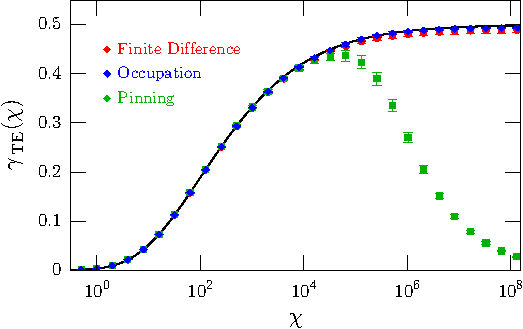
\includegraphics[width=0.6\columnwidth]{fig/numerics/force}
  \caption[Numerically computed TE force]{Numerically computed TE force for pinning (squares), occupation (circles)and finite difference (squares)methods.
    The pinning method fails for the strong coupling limit as a result of the integrand only being nonzero if 
    the path has fine enough resolution.
    The finite difference had the optimal finite difference step $\delta=d/\sqrt{N}$.
    Simulations had $N=10^4$ points per path, with $10^8$ trajectories.}
  \label{fig:force}
\end{figure}
In Fig.~\ref{fig:force}, we plot the numerically calculated force on two dielectric slabs of equal dielectric
constant, normalized to the total EM force between perfect-conducting plates.  This was carried out for both the pinning, occupation
and finite-difference methods.  In all cases, we generate paths using the v-loop algorithm~(\ref{eq:unit_vloop}),
and evaluatethe dielectric path averages using the trapezoidal method discussed in Sec.~\ref{sec:trapezoid}.
Note that in computing path averages for the occupation method, only points \emph{inside} the body
contribute --- any points pinned to lie on the surface do not contribute to the dielectric path-average.

The pinning methods discussed in Sec.~\ref{sec:path-pinning} start to fail for $\chi\sim N$, as expected.
For $\chi\gg N$, the estimate of the force shows the expected $\chi^{-1/2}$ decay.  
For a finite susceptibility, it should be possible to carry out the simulation for large enough $N$, 
but if one is interested in the strong coupling limit of this theory, then the pinning method is unsuitable.

In contrast, the occupation method is better behaved in the strong-coupling limit.  The occupation method estimate for 
the force is computed by generating a fiducial path $\{\vect{y}_k\}$, and translating the path to 
$\vect{x}_k=\vect{y}_k-\vect{y}_j+\vect{d}$, so that that each point $\vect{x}_j$ has a chance to start 
on the surface.  The results are then averaged over all such pinnings. 
However, naively implementing this method leads to $N$ evaluations of the path integral, which could
become a prohibitive amount of work.  
It may be possible to capture both strong and weak coupling limits with only two samples.
First, to capture the strong coupling limit, the path integral can be computed for a path where only one point is on the first surface,
and no points are inside the first body.
Second, to capture the remaining $\chi$-dependence, recompute the path integral for a path where a 
randomly selected point is pinned lie on the first surface, with no regard for the other occupation numbers.
The strong coupling estimate for the force $f_s$, and the 
generic coupling estimate $f_g$, are combined with weights $N^{-1}$ and $(N-1)/N$ respectively, which
account for enforcing the restrictions.

In the absence of that first sampling step, only very rare paths will contribute, since most random paths
starting at the origin are equally like to explore both positive and negative regions. 
Most paths will intersect both bodies, and contribute zero to the force.  For modest ensembles
this causes similar convergence problems to the pinning methods at large $\chi$. 
However, this would be a statistical artifact due to insufficient sampling, rather than due to the 
intrinsic problems in the pinning method.  Similar methods will be discussed in more detail
regarding the potential curvature.  

In fact, the generic samples were gathered using stratified sampling, where the index $k$ was broken into
uniform strata, each of which is sampled from unifromly.  In the simulations in Fig.~\ref{fig:force},
ten strata were used.  
% The occupation method also has an advantage in that there are no explicit tuning parameters, unlike the finite
% difference.   

Given the deficiencies of the pinning method for finite paths, we will compute the potential
curvature using the occupation method.  
Since the potential curvature requires paths pinned on two different surfaces, 
and will exhibit similar convergence issues at strong coupling, we will develop both a generic-coupling
and strong-coupling approach to generating paths and sampling times.  

\subsection{Direct Path Construction for Potential Curvature}
\label{sec:direct_construct}
In a method suitable for generic-coupling, all of the paths start on the first body,
and are explicitly constructed to intersect the second body after $k$ steps, where the index $k$ is also sampled randomly.  
The paths can be explicitly constructed as Brownian bridges from $x=0$ to $x_k=d$, via the open v-loop
algorithm~(\ref{eq:open_vloop}).
The Gaussian factor $\mathcal{G}\big[d,k(N-k)\cT/N^2\big]$ in Eq.~(\ref{eq:curvature_occupy}) is used
to sample path times by treating it as the Gamma distribution.  Path times can be sampled 
from Eq.~(\ref{eq:expT}), with $\cT_0=N^2d^2/[2k(N-k)]$ and $\alpha=1+(D+1)/2$.
% The fixed index $k$ for the pinning is determined by randomly selecting from the resulting
% normalization constant.  
% This can be done efficiently by introducing $u:=\cT_0/\cT$, and noting that $u$ is Gamma distributed,
% \begin{equation}
%   P(u;\alpha) = \frac{u^{\alpha-2}}{\Gamma[\alpha-1]}e^{-u}.
% \end{equation}
% This technique can also be used more generally in worldline path integrals where 
% $\alpha$ is either a small integer or half-integer, and deviates can be easily generated
% as a sum of exponential deviates (and a Gaussian random variable for half-integer values)~\cite{Devroye2003}.
% For the case of two-planar surfaces a distance $d$ apart, , 
% and for the second derivative of the potential .
The pinned point $k$ can be sampled from the combination of $\cT_0^{1-\alpha}$ for normalization $P(\cT)$
and the normalization constant from $\mathcal{G}(d,k(N-k)\cT/N^2)$,  with distribution
\begin{equation}
  P(k;N)=c'_N \bigg(\frac{k(N-k)}{N^2}\bigg)^{\alpha-1-1/2},
\end{equation}
where $c'_N = \sum_{k=1}^NP(k;N)\approx 1/30$ for large $N$.  
In addition for planar surfaces, the integral over the transverse area for 
can be carried out, since it is a simple Gaussian integral decoupled from the other integrals.  

The final expression for the potential curvature is
\begin{align}
  C_{ij}%   =& \frac{\hbar c}{2(2\pi)^{D/2}}\sum_{j,\Delta>0}\int \frac{d\cT}{\cT^{1+D/2}}\biggdlangle \int d\vect{x}_0
%   \frac{N^2e^{-N^2d^2/[2 \Delta(N-\Delta)\cT]}}{\sqrt{2\pi \cT \Delta(N-\Delta)}}\nonumber\\
%   &\times
%    \hat{n}_1(\vect{x}_j)\hat{n}_2(\vect{x}_{k})
%    \sum_{n=0}^{N-2}\sum_{m=0}^{N-n-2}\I[1]n\I[2]m g_{m,n}
%    \biggdrangle_{\vect{x}(\cT);{\sigma_1(\vect{x}_j-\vect{R}_1)=0\atop \sigma_2(\vect{x}_{j+\Delta}-\vect{R}_2)=0}}\\
% =& \frac{\hbar c}{2(2\pi)^{D/2}}\sum_{j}\int d\vect{x}_0\biggdlangle 
% \frac{2^{s-1}\Gamma(s-1)S_{N-1}}{\sqrt{2\pi}|\vect{x}_j-\vect{x}_{j+\Delta}|^{2(s-1)}}
%   \hat{n}_1(\vect{x}_j)\hat{n}_2(\vect{x}_{k})
%   \sum_{n=0}^{N-2}\sum_{m=0}^{N-n-2}\I[1]n\I[2]m g_{m,n}
%   \biggdrangle_{\Delta,\cT,\vect{x}(\cT);{\sigma_1(\vect{x}_j-\vect{R}_1)=0\atop \sigma_2(\vect{x}_k-\vect{R}_2)=0}},
=& \frac{\hbar c N }{2(2\pi)^{D/2}}\oint\limits_{\sigma_1(\vect{x}_0-\vect{R}_1)=0} \hspace{-4ex} dS_0\,\biggdlangle 
\oint\limits_{\sigma_2(\vect{x}_\Delta-\vect{R}_2)=0} \hspace{-4ex} dS_\Delta\,\frac{3c'_{N}\hat{n}_1(\vect{x}_j)\hat{n}_2(\vect{x}_{k})}{|\vect{x}_0-\vect{x}_{\Delta}|^{5}}
  \nonumber\\
  &\hspace{2cm} \sum_{n=0}^{N-2}\sum_{m=0}^{N-n-2}\I[1]n\I[2]m g_{m,n}
  \biggdrangle_{\Delta,\cT,\vect{x}_0\leftrightarrow\vect{x}_\Delta},
\end{align}
where the ensemble average is over path times, pinning separations $\Delta$, and 
Brownian bridges from $\vect{x}_0$ to $\vect{x}_\Delta$, where $\vect{x}_0$ is on the first 
surface, and $\vect{x}_\Delta$ is on the second surface.
% we have used $\dlangle \cdots\drangle_{y; C}$ to denote ensemble averaging over quantities 
% $y$ subject to possible constraints $C$.  The first pinning position is fixed on the first surface,
% the second pinnings are sampled from $P_\Delta$ with $k=j+\Delta$, 
The path times are sampled from $P_{\text{exp-T}}[\cT;\cT_0,1+(D+1)/2]$, with $\cT_0$ given by 
\begin{equation}
  \cT_0 = \frac{N^2d^2}{2\Delta(N-\Delta)} \label{eq:T0_curvature}.
\end{equation}
The paths are still then constructed subject to the constraints of touching the bodies at the appropriate
indices.  The remaining integrand is evaluated for the resulting paths.  

In Fig.~\ref{fig:curvature_a}, we have used this generic-coupling method to compute the potential curvature
without special treatment for strong coupling, with two different ensemble sizes to show the effect of more averaging.  
%Fig.~\ref{fig:curvature_a} shows improved convergence at large $\chi$ once the sample size is increased.  
While the generic-coupling integrand leads to the correct answer in the strong-coupling limit once enough
averaging has been done, this does require a large ensemble to capture relatively rare paths that just graze both surfaces.
Performance can be improved by introducing separate estimates for the strong-coupling limit.  

This suggests a two-fold approach: generate paths constrained to touch without regard for their
occupation time (which will capture small $\chi$), and also isolate a subset of paths which just touch the 
bodies (which will capture large $\chi$).  


\begin{figure}
  \centering
  \includegraphics[width=0.6\columnwidth]{fig/numerics/curvature_a}
  \caption[Numerical TE Potential Curvature for two planar surfaces, evaluated with occupation method]{
    Numerically computed second derivative of potential for two planar surfaces as function 
    of dielectric, for $N=10^5$, each with $10^7$ and $10^9$ trajectories.  
    % While the integrand produces the correct result, recovering the correct answer relies on having a large enough ensemble of 
    % paths, since the strong-coupling limit comes from rare paths.  
    All results are computed using the ``occupation'' method with generic pinning presented in Eq.~\ref{eq:curvature_occupy}.}
\label{fig:curvature_a}
\end{figure}

\subsection{Softened $\delta$-function Pinning for Strong Coupling Limit for Potential Curvature}

An alternative method, more suited to the strong-coupling limit, arises by treating the second $\delta$-function
differently.  
Consider the $j$th term in the potential curvature~\ref{eq:curvature_occupy}, where the second 
$\delta$-function pins a coordinate $\vect{y}_j$ to the second body. 
\begin{align}
  I&=\int d\vect{y}_j \mathcal{G}(\vect{x}_{j+1}-\vect{y}_j,\Delta\cT)
  \mathcal{G}(\vect{y}_{j}-\vect{x}_{j-1},\Delta\cT)\delta[\sigma_2(\vect{y}_j)]f(\vect{y}_j),
\end{align}
where $f$ also depends on all of the other variables.  
As before, the $\delta$-function integrand can evaluated.  However, this time we insert unity,
by multiplying and dividing by the unconstrained integral over the Gaussian probability density for 
path increments from $\vect{x}_{j-1}\rightarrow\vect{x}_j$ and $\vect{x}_{j}\rightarrow\vect{x}_{j+1}$,
\begin{align}
  I&=\int d\vect{y}_j \mathcal{G}(\vect{x}_{j+1}-\vect{y}_j,\Delta\cT)
  \mathcal{G}(\vect{y}_{j}-\vect{x}_{j-1},\Delta\cT)\delta[\sigma_2(\vect{y}_j)]f(\vect{y}_j)\nonumber\\
  &=\hspace{-1ex}\oint\limits_{\sigma_2(\vect{y}_j)=0}\hspace{-2ex}dS_j\,
  \frac{f(\vect{y}_j)}{|\nabla\sigma_2(\vect{y}_j)|}
  \frac{\mathcal{G}(\vect{x}_{j+1}-\vect{y}_j,\Delta\cT)\mathcal{G}(\vect{y}_{j}-\vect{x}_{j-1},\Delta\cT)}
  {\mathcal{G}(\vect{x}_{j+1}-\vect{x}_{j-1},2\Delta\cT)}\nonumber\\
  &\hspace{0.5cm}\times \bigg[\int d\vect{x}_j\,
  \mathcal{G}(\vect{x}_{j+1}-\vect{x}_j,\Delta\cT)\mathcal{G}(\vect{x}_{j}-\vect{x}_{j-1},\Delta\cT)\bigg].
\end{align}
This can be used inside the path integral, and since the integral over $\vect{x}_j$ is unconstrained, 
ree Brownian paths can be constructed using the introduced integral $\vect{x}_j$.  
The pinned coordinate $\vect{y}_j$ is now relegated to an additional integral.
This has in effect softened the $\delta$-constraint, since
the integral over $\vect{y}_j$ is only significant for paths that pass within $\pm\sqrt{\Delta\cT}$ of the constraint surface.
One downside of this approach is that there is an additional $(\Delta\cT)^{-1/2}$ factor from the constrained Gaussian factors.
This factor can be absorbed if we treat the combined constrained Gaussian factors as the probability
distribution for $\cT$.  We would then effectively sample from paths that are nearly contacting the surface,
and with a greater probability of finding paths that have \emph{not} entered into the body.  

For a particular starting point $\vect{x}_0$, pinning point $\vect{y}$, and path $\vect{x}_j=\vect{x_0}+\sqrt{\cT}\vect{B}_j$,
the combined Gaussian factor involving $\vect{x}_{j\pm 1},\vect{y}$ can be converted into a probability distribution for
the allowed times, $\cT$.  The combined Gaussian can be written as 
\begin{equation}
 \frac{\mathcal{G}(\vect{x}_{j+1}-\vect{y}_j,\Delta\cT)\mathcal{G}(\vect{y}_{j}-\vect{x}_{j-1},\Delta\cT)}
  {\mathcal{G}(\vect{x}_{j+1}-\vect{x}_{j-1},2\Delta\cT)} = \frac{1}{(\pi\Delta\cT)^{D/2}}e^{-Y}
\end{equation}
where 
\begin{align}
 Y&=\frac{(\vect{x}_{j+1}-\vect{y}_j)^2}{2\Delta\cT}+\frac{(\vect{y}_j-\vect{x}_{j-1})^2}{2\Delta\cT}
-\frac{(\vect{x}_{j+1}-\vect{x}_{j-1})^2}{4\Delta\cT}\nonumber\\
  &= N|\vect{y}_j-\vect{x}_0|^2\bigg(\frac{1}{\sqrt{\cT}} -\frac{(\vect{y}_j-\vect{x}_0)\cdot\bar{\vect{B}}_j}{|\vect{y}_j-\vect{x}_0|^2}\bigg)^2
%\nonumber\\  &\hspace{0.5cm}
  \hspace{-1mm}+N\hspace{-1mm}\left[\bar{\vect{B}}_{j}^2-\frac{[(\vect{y}_j-\vect{x}_0)\cdot\bar{\vect{B}}_j]^2}{|\vect{y}_j-\vect{x}_0|^2}\right]
\end{align}
where $\bar{\vect{B}}_j:=(\vect{B}_{j+1}+\vect{B}_{j-1})/2$ is the mean value of the neighboring bridge
points.  
The first factor is effectively Gaussian in $1/\sqrt{\cT}$.  The second factor suppresses terms where the 
$\bar{B}_j$ is pointed in the wrong direction, i.e. away from the starting point $\vect{x}_0$ and the desired
point of the surface $\vect{y}_j$.
The second term is zero for the planar geometries.  
%This second factor could in turn be used to sample from the surface for a given path.  
In essence, this method for handling the $\delta$-function has replaced the $\delta$-function 
with a softer distribution that allows paths within $\pm N^{-1/2}$ of the required times and positions.  

The potential curvature can be split into two terms, one involving just the strong-coupling limit
$g_{0,0}$ where paths do not enter the bodies, and another with all of the remaining terms.   
The second term can be sampled using the generic coupling algorithm from Sec.~\ref{sec:direct_construct}.
These will be evaluated separately, although they may share random numbers. 

In order to capture the strong-coupling dependence it is necessary to also sample from the no-touching
set of paths.  For two half-spaces this can be constructed by shifting paths so that the minimum
point of the path starts on one body, $B(t)\rightarrow B(t) -B_{\text{min}}+d_1$.
We then find the maximum point $B_{\text{max}}$ and consider finding the path times when 
that point is close to the second surface $d_2$.
Let us call the index of the maximum location $j$.

The leading exponential potential can be converted into a probability distribution for $\cT$ on a 
path-wise basis if we consider $x_j = x_0+\sqrt{\cT}B_j$, where $B_j$ is the $j$th coordinate of a 
unit Brownian bridge.   The exponential factor can be written as 
\begin{align}
  \exp\bigg(-\frac{1}{\Delta \cT}[d-(x_{j+1}+x_{j-1})/2]^2/\Delta \cT\bigg) 
  &= \exp\bigg(-Nd^2\bigg(\frac{1}{\sqrt{\cT}}-\frac{\bar{B}_j}{d}\bigg)^2\bigg],
\end{align}
where $\bar{B}_j := (B_{j+1}-B_{j-1})/2$.  This is effectively a Gaussian in $1/\sqrt{\cT}$.  
The normalized probability distribution for $1/\sqrt{\cT}$ is  
\begin{equation}
  P_C(\cT;\bar{B}_j,d,N) = \sqrt{\frac{Nd^2}{\pi\cT^3}}\exp\bigg[-Nd^2\left(\frac{1}{\sqrt{\cT}}-\frac{\bar{B}_j}{d}\right)^2\bigg],
\label{eq:time_fix_curve}
\end{equation}
for $\cT\in[0,(d/\bar{B}_j)^2]$. 
The probability distribution can be converted to an one-sided normal distribution by defining
\begin{equation}
  s = \sqrt{2Nd^2}\left(\frac{1}{\sqrt{\cT}}-\frac{\bar{B}_j}{d}\right),
\end{equation}
In that case, $s$ is the absolute value of a standard normal deviate, and 
the path times are then given by
\begin{equation}
  \cT = \left( \frac{|z|}{\sqrt{2Nd^2}}+\frac{\bar{B}_j}{d}\right)^{-2}\label{eq:cT-s},
\end{equation}
where $z$ is a standard-normal deviate.  
With the above method of handling the $\delta$-function, there is no need for an additional Gaussian
pinning factor for planar surfaces.  

The potential curvature can be sampled from this set of paths as
\begin{align}
  C^{(S)}_{ij}  =& \frac{N\hbar c}{2(2\pi)^{D/2}}\biggdlangle \int_0^\infty \frac{d\cT}{\cT^{1+D/2}}
  \sum_k \int dy_k \frac{e^{-(y_k-\bar{B}_k)^2/\Delta \cT}}{(\pi\Delta\cT)^{1/2}}
   e^{(d-\bar{B}_k)^2/\Delta \cT}\I[1]0\I[2]0 g_{0,0}
   \biggdrangle_{x(\cT)}.
 \end{align}
The $\cT$ integral will be solved in Monte Carlo fashion after factoring out the probability density~(\ref{eq:time_fix_curve}),
and using Eq.~(\ref{eq:cT-s}).  The integral can be cut off at $\cT_0:=(d/\bar{B}_k)^2$, since for $\cT>\cT_0$
more than one point has definitely entered the bodies. 
In strong-coupling, only the no-touching terms contribute, and we can use $g_{0,0}=1$.
\begin{align}
C^{(S)}_{ij} =& \frac{N\hbar c}{2(2\pi)^{D/2}}\biggdlangle  \frac{1}{\cT^{1+D/2}}
  \sum_k   \sqrt{\frac{\pi\cT^3}{Nd^2}}\sqrt{\frac{N}{\pi\cT}}
   \I[1]0\I[2]0 
   \biggdrangle_{\vect{x}(\cT), \cT}\\
 =& \frac{N\hbar c}{2(2\pi)^{D/2}}\biggdlangle  \frac{1}{\cT^{D/2}}
  \sum_k  \frac{1}{d}   \I[1]0\I[2]0 
   \biggdrangle_{\vect{x}(\cT), \cT}.
\end{align}
Note that there are no explicit restrictions on the paths, but the integral is only significant
when the paths are pass close to the body.
(For planar surface, the Gaussian integrals over $\vect{y}$ can be carried out, 
while it is necessary to factor out the cross-sectional area, and consider the second derivative 
of the energy per unit area).



\begin{figure}
  \centering
  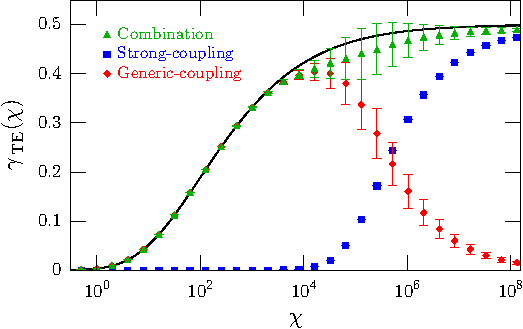
\includegraphics[width=0.6\columnwidth]{fig/numerics/curvature_c}
  \caption[Numerical TE Potential Curvature for two planar surfaces, evaluated with strong-coupling methods]{Numerically computed second derivative of TE potential for two planar surfaces as function 
    of dielectric, for $N=10^5$, with $10^8$ trajectories.
    Strong-coupling results are shown as blue squares, generic coupling as red diamonds, 
    and their sum as green triangles.  
    All simulations are computed using
  ``occupation'' method in Eq.~\ref{eq:curvature_occupy}, and come from the same ensemble.}
\label{fig:curvature_c}
\end{figure}

Fig.~\ref{fig:curvature_c} shows the inclusion of the strong-coupling term.  It only becomes important for $\chi/N\gg 1$,
and there is a transition between the generic coupling, and strong-coupling results.  Carrying out 
further averaging of course improves the results.   The variance is also increased in the cross-over region.


%\section{Numerical Implementation for TE Potential Curvature}

% The path integral for the potential curvature in the occupation numbers approach requires paths 
% that are constrained by $\sigma_1(\vect{x}_j)$ and $\sigma_2(\vect{x}_k)$.  
% There are a couple approaches to take here.  First, we could generate paths and then retroactively
% find points close to the requisite surfaces, and perturb those paths such that the points do touch the 
% surface.  We would then sum over all possible combinations of the indices close to the surfaces.
% In this approach we would sample a position $x_0$, and then a time $\cT$.  Then we would find the 
% near-intersections, and sum the integral over perturbing these.  

% Recall, the potential curvature is 
% \begin{align}
%   C_{ij} =& \frac{\hbar c N}{2(2\pi)^{D/2}}\intzinf\frac{d\cT}{\cT^{1+D/2}}
%   \hspace{-2ex}\oint\limits_{\sigma_2(\vect{x}_0-\vect{R}_2)=0}  \hspace{-4ex} dS_0\, \hat{n}_1(\vect{x}_0)
%   %\nonumber\\ 
% %  &\times
% \biggdlangle 
%   \sum_{k=0}^{N-1}\hat{n}_2(\vect{x}_k)\mathcal{G}(\vect{x}_0,\vect{x}_k,k,\cT)
%   \nonumber\\
%   &\hspace{0.75cm} \times\sum_{n=0}^{N-2}\sum_{m=0}^{N-n-2}\I[1]n\I[2]m g_{m,n}
%   \biggdrangle_{\vect{x}(t)|\sigma_2(\vect{x}_k-\vect{R}_2)=0}
% \end{align}
% where 
% \begin{align}
%   g_{m,n}=c_{m+1,n+1}+c_{m,n}-c_{m+1,n}-c_{m,n+1},
% \end{align}

% That effort scales quite badly roughly as an additional $N^2$.  
% We could pick the a pair of fixed indices based on their probability of occurring?  
% Secondly, we could also explicitly sample from the strong-coupling limit.

% This integrand is non-zero for paths that touch both bodies.  In the strong-coupling limit,
% only paths that just graze the bodies will contribute.  However at finite $\chi$, all paths 
% are useful since paths with a finite sojourn time contribute significantly.  


% We can either directly generate the paths that obey the constraints, or we can generate 
% generic paths and then check whether these paths touch the desired surfaces.  

% In the second strategy, the paths are generated, and we then check if there are any points
% on the path which are close to a surface.  Mathematically 
% $\text{min}_x|\vect{x}_j-\sigma_i(x)|\sim \sqrt{\Delta T}$.  We would then find all such points
% for both bodies and then randomly select a pair to be pinned to the surface.
%  We would also have to introduce the correction
% for distorting this path point to lie on the surface,
% \begin{equation}  
%   P_{\text{pin-corr}} = \frac{P_{\text{pinned}}}{P_{\text{free}}}
%   =\frac{ e^{-|\vect{x}_{j+1}-\vect{x}^*|^2/(2\Delta T)-|\vect{x}_{j-1}-\vect{x}^*|^2/(2\Delta T)  } }
%   {e^{-|\vect{x}_{j+1}-\vect{x}_j|^2/(2\Delta T)-|\vect{x}_{j-1}-\vect{x}_j|^2/(2\Delta T)  }},
% \end{equation}
% where $x^*$ is the nearest point to the surface to $\vect{x}_j$.

%\subsection{Softened $\delta$-function}
% There is an alternative formulation for handling the $\delta$-function.  Instead of explicitly constructing 
% paths to satisfy the $\delta$-function, we can generate an effective potential.  
% First consider a single integral against a Gaussian distribution, with a $\delta$-function,
% \begin{align}
%   I &= \int dx_j \frac{1}{2\pi\Delta\cT}
%   e^{-(x_{j+1}-x_j)^2/(2\Delta \cT)-(x_{j}-x_{j+1})^2/(2\Delta \cT)} f(x_j)\delta(x_j-d) \\
% &=
% \frac{1}{2\pi\Delta\cT}
%   e^{-(x_{j+1}-d)^2/(2\Delta \cT)-(d-x_{j+1})^2/(2\Delta \cT)} f(d).
% \end{align}
% While this integral can be straightforwardly evaluated, it is inconvenient within the path integral
% to have to sum over explicitly pinned paths for each $x_j$.  We can circumvent this by inserting unity 
% by multiplying and dividing by an integral over the Gaussian probability distribution, 
% \begin{align}
%   I &= \frac{1}{2\pi\Delta\cT}
%   e^{-(x_{j+1}-d)^2/(2\Delta \cT)-(d-x_{j+1})^2/(2\Delta \cT)} f(d)
%   \nonumber\\  &\times
% \dfrac{\int dy_j (2\pi\Delta\cT)^{-1}
%   e^{-(x_{j+1}-y_j)^2/(2\Delta \cT)-(y_{j}-x_{j+1})^2/(2\Delta \cT)}}{\int dy_j (2\pi\Delta\cT)^{-1}
%   e^{-(x_{j+1}-y_j)^2/(2\Delta \cT)-(y_{j}-x_{j+1})^2/(2\Delta \cT)}}\\
% % &= \frac{1}{2\pi\Delta\cT}
% %   e^{-(x_{j+1}-d)^2/(2\Delta \cT)-(d-x_{j+1})^2/(2\Delta \cT)} f(d)
% %   \left[\frac{1}{\sqrt{4\pi\Delta \cT}}e^{-(x_{j+1}-x_{j-1})^2/(4\Delta\cT)}\right]^{-1}
% % \nonumber\\
% % &\times\int dy_j \frac{1}{2\pi\Delta\cT}
% %   e^{-(x_{j+1}-y_j)^2/(2\Delta \cT)-(y_{j}-x_{j+1})^2/(2\Delta \cT)}\\
% &= \frac{1}{\sqrt{\pi\Delta\cT}}
%   e^{-[d-(x_{j+1}+x_{j-1})/2]^2/\Delta \cT}f(d)
% \int dy_j \frac{1}{2\pi\Delta\cT}
%   e^{-(x_{j+1}-y_j)^2/(2\Delta \cT)-(y_{j}-x_{j+1})^2/(2\Delta \cT)}.
% \end{align}
% In the path integral one can then use free paths, where the introduced coordinate
% $y_j$ replaces the constrained $x_j$ coordinate, and is subsumed within the free Gaussian path measure.
% The downside is that the integrand is only non-zero
% for a small range of times and positions, but this can be taken into account in the Monte Carlo sampling
% strategy.  

% This can be extended to handle multi-dimensional paths subject to a surface constraint, $\delta[\sigma(\vect{x})]$.
%  In that case 
% one multiplies and divides by the appropriate multi-dimensional Gaussian.  Since each Cartesian dimension
% of the Gaussians decouples from the others, the same manipulations apply dimension-by-dimension, 
% with the result
% \begin{align}
%   I % &= \int_{\sigma(\vect{y})=0}dS\frac{1}{|\nabla\sigma|}\frac{1}{(2\pi\Delta\cT)^D}
% %   e^{-|\vect{x}_{j+1}-\vect{y}|^2/(2\Delta \cT)-|\vect{y}-\vect{x}_{j+1}|^2/(2\Delta \cT)} f(\vect{y})
% %   \nonumber\\  &\times
% % \dfrac{\int d\vect{x}_j \dfrac{1}{(2\pi\Delta\cT)^{D/2}}
% %   e^{-|\vect{x}_{j+1}-\vect{x}_j|^2/(2\Delta \cT)-|\vect{x}_{j}-\vect{x}_{j-1}|^2/(2\Delta \cT)}}
% % {\int d\vect{x}_j \dfrac{1}{(2\pi\Delta\cT)^{D/2}}
% %   e^{-|\vect{x}_{j+1}-\vect{x}_j|^2/(2\Delta \cT)-|\vect{x}_{j}-\vect{x}_{j-1}|^2/(2\Delta \cT)}}\\
% % &= \frac{1}{2\pi\Delta\cT}
% %   e^{-(x_{j+1}-d)^2/(2\Delta \cT)-(d-x_{j+1})^2/(2\Delta \cT)} f(d)
% %   \left[\frac{1}{\sqrt{4\pi\Delta \cT}}e^{-(x_{j+1}-x_{j-1})^2/(4\Delta\cT)}\right]^{-1}
% % \nonumber\\
% % &\times\int dy_j \frac{1}{2\pi\Delta\cT}
% %   e^{-(x_{j+1}-y_j)^2/(2\Delta \cT)-(y_{j}-x_{j+1})^2/(2\Delta \cT)}\\
% % &= \int_{\sigma(\vect{y})=0}dS\frac{1}{|\nabla\sigma|}\frac{1}{(\pi\Delta\cT)^{D/2}}
% %   e^{-|\vect{x}_{j+1}-\vect{x}_{j-1}|^2/(4\Delta \cT)-|\vect{x}_{j+1}-\vect{y}|^2/(2\Delta \cT)-|\vect{y}-\vect{x}_{j+1}|^2/(2\Delta \cT)} f(\vect{y})\nonumber\\
% %   &\times\int d\vect{x}_j \frac{1}{(2\pi\Delta\cT)^{D/2}}
% %   e^{-|\vect{x}_{j+1}-\vect{x}_j|^2/(2\Delta \cT)-|\vect{x}_{j}-\vect{x}_{j-1}|^2/(2\Delta \cT)}\\
% =& \int_{\sigma(\vect{y})=0}dS\frac{1}{|\nabla\sigma|}\frac{1}{(\pi\Delta\cT)^{D/2}}
%   e^{-|\vect{y}-(\vect{x}_{j+1}+\vect{x}_{j-1})/2|^2/(\Delta \cT)} f(\vect{y})\nonumber\\
%   &\times\int d\vect{x}_j \frac{1}{(2\pi\Delta\cT)^{D/2}}
%   e^{-|\vect{x}_{j+1}-\vect{x}_j|^2/(2\Delta \cT)-|\vect{x}_{j}-\vect{x}_{j-1}|^2/(2\Delta \cT)}.
% \end{align}

% This allows us to use paths that are close to the surface, without exactly touching the surface.  
% The integrand is still only significant for times and paths where this occurs.  For a fixed 
% starting point $\vect{x}_0$, pinning point $\vect{y}$, and path $\vect{x}_j=\vect{x_0}+\sqrt{\cT}\vect{B}_j$,
% this can be converted into a probability distribution for
% the allowed times, $\cT$.    
% \begin{align}
%   \exp\bigg[-\frac{|\vect{y}-(\vect{x}_{j+1}+\vect{x}_{j-1})/2|^2}{\Delta\cT}\bigg]
%   &= \exp\bigg[-\frac{1}{\Delta\cT}|\vect{d}-\sqrt{\cT}\bar{\vect{B}}_{j}|^2\bigg] \\
%   &= \exp\bigg[-N\bigg(\frac{\vect{d}^2}{\cT} -\frac{2\vect{d}\cdot\bar{\vect{B}}_j}{\sqrt{\cT}}
%     + \bar{\vect{B}}_{j}^2\bigg)\bigg] \\
%   &= \exp\bigg[-N|\vect{d}|^2\bigg(\frac{1}{\sqrt{\cT}} -\frac{\vect{d}\cdot\bar{\vect{B}}_j}{|\vect{d}|^2}\bigg)^2
% %  \bigg]  \nonumber\\    &\times\exp\bigg[
%     -N\left(\bar{\vect{B}}_{j}^2-\frac{(\vect{d}\cdot\bar{\vect{B}}_j)^2}{|\vect{d}|^2}\right)\bigg] 
% \end{align}
% where we introduce $\bar{\vect{B}}_j:=(\vect{B}_{j+1}+\vect{B}_{j-1})/2$ and $\vect{d}=\vect{y}-\vect{x}_0$.
% The first factor is effectively Gaussian in $1/\sqrt{\cT}$, while the second factor suppresses terms where the 
% path is orthogonal to line between the path starting point, and the patch on the surface.  
% This second factor could in turn be used to sample from the surface for a given path.  
%\subsection{Direct Construction of constrained paths}

% Alternatively,  we can enforce the touching constraint directly and make the paths touch the bodies by constructing
% paths which are fixed at steps $j$ and $k$ to touch the surface, and sum over all $j,k\in {1,N}$.  
% Evidently the direct approach will create many paths with small contributions, particular if $j-k \sim 1$.
% This can be made more efficient by exploiting the Gaussian factor as a probability distribution.

% In computing the energy the Gaussian is introduced for the purpose of importance sampling, and must
% be factored out.  In this case, the Gaussian factor is already manifest, and should be taken into account
% when sampling time.s   
% We would sample times from Eq.~\ref{eq:expT}, with 
% \begin{equation}
%   T_0 = \frac{N^2d^2}{2\Delta(N-\Delta)} \label{eq:T0_curvature}
% \end{equation}
% where $\Delta$ is the difference in indices at the crossing points.
% The result of using this is as our probability distribution is to factor out a normalization constant,
% which leaves the integrand as 
% \begin{equation}
%   c=\frac{N}{\sqrt{2\pi\Delta(N-\Delta)}}\Gamma(s-1)\bigg(\frac{N^2d^2}{2\Delta(N-\Delta)}\bigg)^{-s+1}
%     =\frac{2^{s-1}\Gamma(s-1)}{\sqrt{2\pi} d^{2s-2}}\bigg[\frac{\Delta(N-\Delta)}{N^2}\bigg]^{s-3/2}
% \end{equation}
% where the exponent $s=1+(D+1)/2=7/2$ accounts for the path integral normalization and the Gaussian factors of $T$ at
% zero temperature.    
% The values for the difference between the pinning indices $\Delta$ are found by numerical root-finding, using bisection.
% The cumulative probability distribution for $\Delta$ is
% \begin{gather}
%  S_\Delta = \frac{1}{S_{N-1}}\sum_{j=1}^\Delta \bigg[\frac{j(N-j)}{N^2}\bigg]^{s-3/2}
% \end{gather}
% Given a uniform random number $u$, the corresponding index $\Delta$ must satisfy $S_{\Delta-1}<u<S_\Delta$.
% The difference $\Delta$ can be found by bisection and starting with estimates at $S_0$ and $S_{N-1}$.






%%% Local Variables: 
%%% mode: latex
%%% TeX-master: "thesis_master"
%%% End: 
